%----------------------------------------------------------------------
\begin{frame}{Cohorts where all are exposed}
When there is no comparison group we may ask:\\
Do mortality rates in cohort differ from those of an
\textbf{external} population, for example:

\pause
Rates from:
\begin{itemize}
\item Occupational cohorts
\item Patient cohorts
\end{itemize}
\pause
compared with reference rates obtained from:
\begin{itemize}
\item Population statistics (mortality rates)
\item Hospital registers (disease rates)
% \item Cancer registers
\end{itemize}
\end{frame}

%----------------------------------------------------------------------
\begin{frame}{Cohort rates vs. population rates: RSR}
  \begin{itemize}
  \item \textbf{Additive:} $\lambda(a) = \delta(a) + \lambda_\text{p}(a)$
  \item Note that the survival (since $a=a_0$, say) is: \vspace*{-1ex}
\begin{align*}
     S(a) &= \exp\Bigl(-\!\!\int_{a_0}^a\!\! \delta(a) + \lambda_\text{p}(a) \dif a\Bigr)\\
          &= \exp\Bigl(-\!\!  \int_{a_0}^a\!\! \delta(a) \dif a\Bigr) \times S_\text{p}(a)\\
    \Rightarrow \quad
    r(a) = S(a)/S_\text{p}(a) &= \exp\Bigl(-\!\!\int_{a_0}^a\!\! \delta(a) \dif a\Bigr)
  \end{align*}

  \item \textbf{Additive} model for \textbf{rates} $\Leftrightarrow$ \textbf{Relative survival} model.
  \end{itemize}
\end{frame}

%----------------------------------------------------------------------
\begin{frame}{Cohort rates vs. population rates: SMR}
  \begin{itemize}
  \item \textbf{Multiplicative:} $\lambda(a) = \theta \times \lambda_\text{p}(a)$
  \item Cohort rates proportional to reference rates, $\lambda_\text{p}$:\\
    $\lambda(a) = \theta \times \lambda_\text{p}(a)$ --- $\theta$ the same in all
    age-bands.
  \item $D_a$ deaths during $Y_a$ person-years an age-band $a$ gives
    the likelihood:
 \begin{eqnarray*}
    D_a \log(\lambda(a)) - \lambda(a) Y_a
  & = & D_a \log(\theta\lambda_\text{p}(a)) - \theta\lambda_\text{p}(a) Y_a \\
  & = & D_a \log(\theta)+ D_a \log(\lambda_\text{p}(a)) % \\ & &
        - \theta(\lambda_\text{p}(a) Y_a)
\end{eqnarray*}
\item The constant $D_a \log(\lambda_\text{p}(a))$ does not involve $\theta$,
  and so can be dropped.
\end{itemize}
\end{frame}

%----------------------------------------------------------------------
\begin{frame}
  \begin{itemize}
  \item $\lambda_\text{p}(a)Y_a = E_a$ is the ``expected'' number of cases in
    age $a$, so the log-likelihood contribution from age $a$ is:
\[
 D_a \log(\theta) - \theta\big(\lambda_\text{p}(a) Y_a\big) =
 D_a \log(\theta) - \theta(E_a)
\]
%% \item \textbf{Note:} $\lambda_\text{p}(a)$ is known for all values of $a$.
\item The log-likelihood is similar to the log-likelihood for a rate, so:
\[
  \hat\theta = \sum_aD_a / \sum_aE_a =
  \mbox{Observed}/\mbox{Expected}
  = \SMR
\]
%% \item $\SMR$ is the maximum likelihood estimator of the relative
%%   mortality in the cohort.
\end{itemize}
\end{frame}

%----------------------------------------------------------------------
\begin{frame}
  \frametitle{Modeling the SMR in practice}
  \begin{itemize}[<+->]
  \item As for the rates, the SMR can be modelled using individual
    data.
  \item Response is $d_i$, the event indicator (\code{lex.Xst}).
  \item $\log$-offset is the expected value for each piece of
    follow-up, $e_i=y_i \times \lambda_\text{p}$ (\code{lex.dur * rate})
  \item $\lambda_\text{p}$ is the population rate corresponding to the age,
    period and sex of the follow-up period $y_i$.
  \end{itemize}
\end{frame}

%----------------------------------------------------------------------
\begin{frame}[fragile]
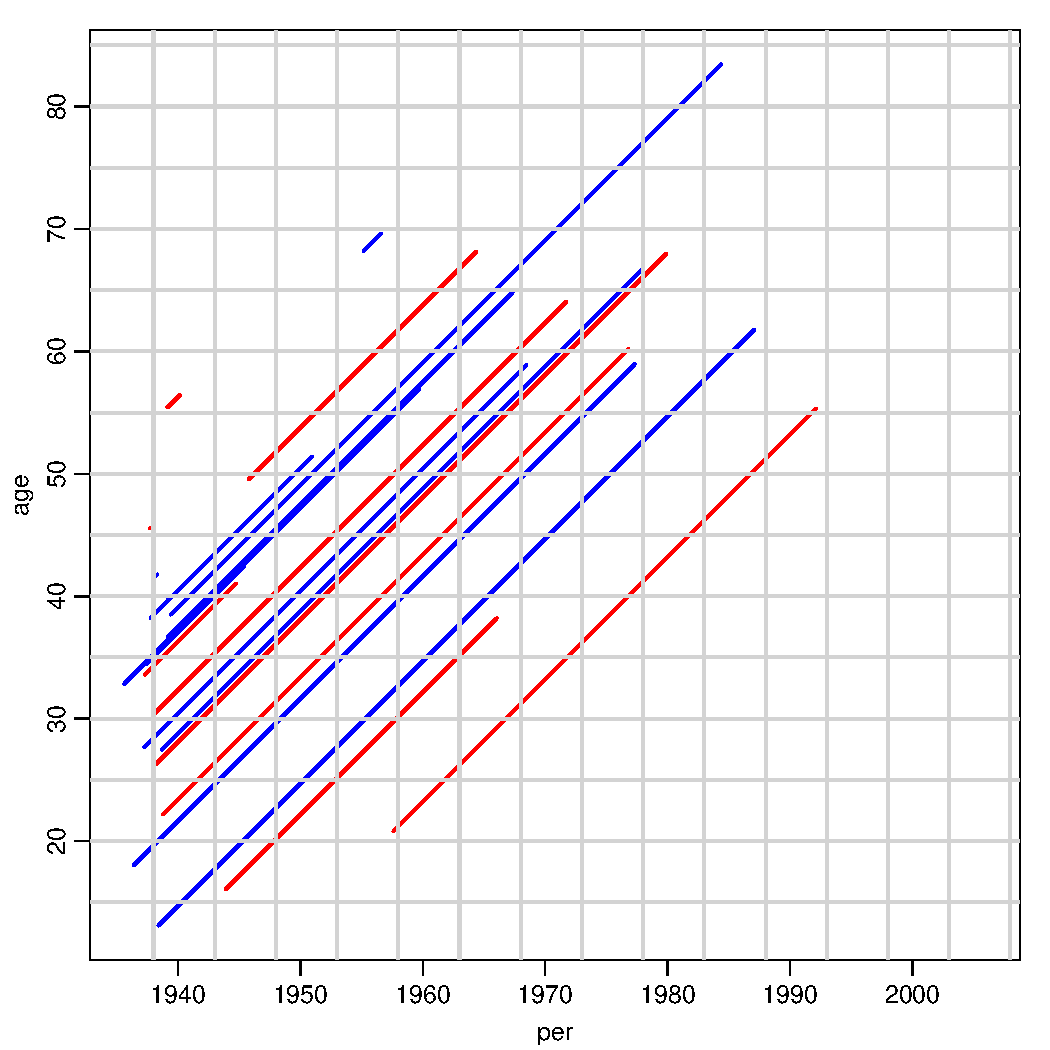
\includegraphics[height=0.99\textheight,keepaspectratio]{thL-lexis3}
\end{frame}

%----------------------------------------------------------------------
\begin{frame}[fragile]
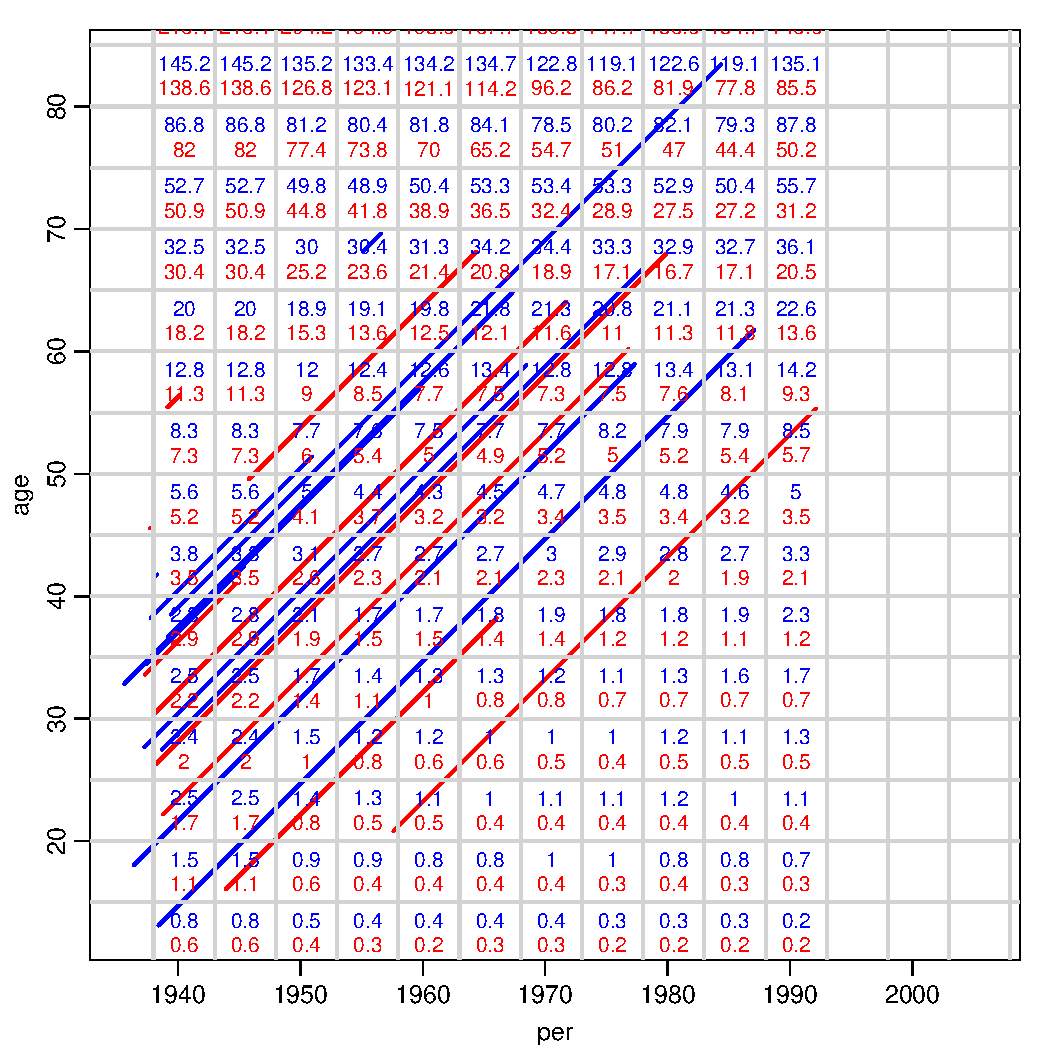
\includegraphics[height=0.99\textheight,keepaspectratio]{thL-lexis4}
\end{frame}

%----------------------------------------------------------------------
\begin{frame}[fragile]{Split the data to fit with population data}
\begin{Schunk}
\begin{Sinput}
> thad <- splitMulti(thL, age=seq(0,90,5), dte=seq(1938,2038,5) )
> summary( thad )
\end{Sinput}
\begin{Soutput}
Transitions:
     To
From     0    1  Records:  Events: Risk time:  Persons:
   0 21059 1939     22998     1939   51787.96      2463
\end{Soutput}
\end{Schunk}
\pause
\vspace*{-1em}
Create variables to fit with the population data
\vspace*{-1ex}
\begin{Schunk}
\begin{Sinput}
> thad$agr <- timeBand( thad, "age", "left" )
> thad$per <- timeBand( thad, "dte", "left" )
> round( thad[1:5,c("lex.id","age","agr","dte","per","lex.dur","lex.Xst","sex")], 2 )
\end{Sinput}
\begin{Soutput}
 lex.id   age     dte lex.dur lex.Xst agr  per sex
      1 22.18 1938.79    2.82       0  20 1938   2
      1 25.00 1941.61    1.39       0  25 1938   2
      1 26.39 1943.00    3.61       0  25 1943   2
      1 30.00 1946.61    1.39       0  30 1943   2
      1 31.39 1948.00    3.61       0  30 1948   2
\end{Soutput}
\end{Schunk}
\end{frame}

%----------------------------------------------------------------------
\begin{frame}[fragile]
\begin{Schunk}
\begin{Sinput}
> data( gmortDK )
> dim( gmortDK )
\end{Sinput}
\begin{Soutput}
[1] 418  21
\end{Soutput}
\begin{Sinput}
> gmortDK[1:6,1:6]
\end{Sinput}
\begin{Soutput}
  agr per sex   risk    dt     rt
1   0  38   1 996019 14079 14.135
2   5  38   1 802334   726  0.905
3  10  38   1 753017   600  0.797
4  15  38   1 773393  1167  1.509
5  20  38   1 813882  2031  2.495
6  25  38   1 789990  1862  2.357
\end{Soutput}
\begin{Sinput}
> gmortDK$per <- gmortDK$per+1900
> #
> thadx <- merge( thad, gmortDK[,c("agr","per","sex","rt")] )
> #
> thadx$E <- thadx$lex.dur * thadx$rt / 1000
\end{Sinput}
\end{Schunk}
\end{frame}

%----------------------------------------------------------------------
\begin{frame}[fragile]
\begin{Schunk}
\begin{Sinput}
> stat.table(contrast,
+            list( D = sum(lex.Xst),
+                  Y = sum(lex.dur),
+                  E = sum(E),
+                SMR = ratio(lex.Xst, E)),
+             margin = TRUE,
+               data = thadx)
\end{Sinput}
\begin{Soutput}
 -------------------------------------------- 
 contrast         D        Y       E     SMR  
 -------------------------------------------- 
 1           917.00 20045.46  214.66    4.27  
 2          1022.00 31742.51  447.21    2.29  
                                              
 Total      1939.00 51787.96  661.87    2.93  
 -------------------------------------------- 
\end{Soutput}
\end{Schunk}
\end{frame}

%----------------------------------------------------------------------
\begin{frame}[fragile]
\begin{Schunk}
\begin{Soutput}
 -------------------------------------------- 
 contrast         D        Y       E     SMR  
 -------------------------------------------- 
 1           917.00 20045.46  214.66    4.27  
 2          1022.00 31742.51  447.21    2.29  
 -------------------------------------------- 
\end{Soutput}
\end{Schunk}
\vspace*{-1em}
\begin{Schunk}
\begin{Sinput}
> m.SMR <- glm(cbind(lex.Xst, E) ~ factor(contrast) - 1,
+              family = poisreg,
+                data = thadx)
> round(ci.exp(m.SMR), 2)
\end{Sinput}
\begin{Soutput}
                  exp(Est.) 2.5% 97.5%
factor(contrast)1      4.27 4.00  4.56
factor(contrast)2      2.29 2.15  2.43
\end{Soutput}
\end{Schunk}
\pause
\begin{itemize}[<+->]
\item Analysis of SMR is like analysis of rates:
\item Replace $Y$ with $E$ --- that's all! (\code{glm.Lexis} not usable)
\item \ldots it's the calculation of $E$ that is difficult
\end{itemize}
\end{frame}
